\subsection{Enakovredni stolpci}

Do sedaj smo obravnavali samo stolpce, ki so imeli enako širino. Kaj pa, če je mogoče optimalna izbira taka, da stolpci niso enako široki? Eden od takih načinov je vpeljava enakovrednih stolpcev.

\begin{definicija}
    Naj bo $S$ množica podatkov. Naj bo $h$ histogram z $n$ stolpci, $n < |S|$, zgrajen glede na podatke iz $S$. Histogram ima \textbf{enakovredne stolpce}, če je v vseh stolpcih "približno enako" število podatkov.
\end{definicija}

\begin{figure}[!h]
    \centering
    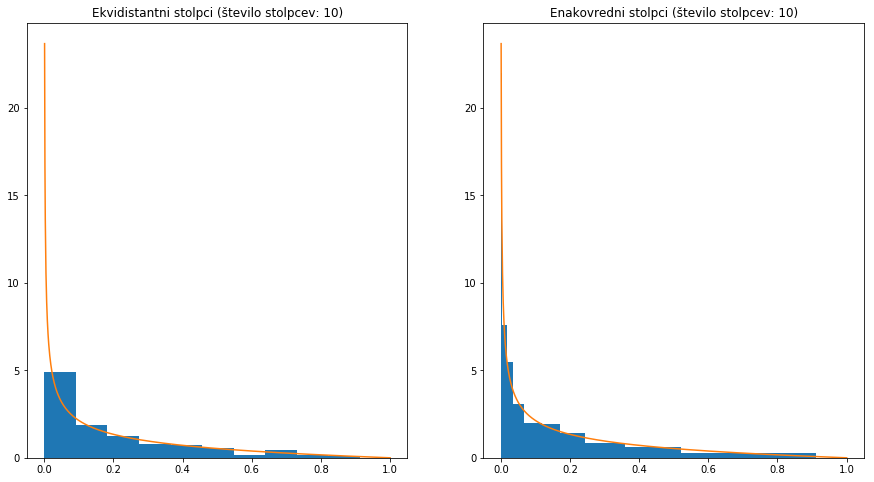
\includegraphics[width=\textwidth]{ekvikvan.png}
    \caption{Primerjava med histogramom z enako širokimi stolpci in histogramom z enakovrednimi stolpci za beta porazdelitev ($\alpha = 0.5$, $\beta = 2$). Vidimo, da se ob istem številu stolpcev veliko bolj prilegajo enakovredni stolpci}
\end{figure}

V zgornji definiciji smo uporabili besedno zvezo "približno enako", ker ni nujno, da je število $|S|$ deljivo s številom $n$. Pri konstrukciji takega histograma pa se temu problemu lahko izognemo recimo tako, da v zadnji stolpec damo toliko podatkov, kolikor je ostanek pri deljenju števila $|S|$ z $n$. Najprej opišimo, kako konstruiramo takšen histogram, nato pa si bomo to pogledali na zgledu.

\subsubsection*{Konstrukcija histograma z enakovrednimi stolpci}

Naj bo $S = \{x_1, x_2, \ldots, x_m\}$ množica podatkov. Konstruirati želimo histogram z $n$ stolpci. Ta histogram bo imel enakovredne stolpce, če bo v vsakem stolpcu $\lfloor m/n \rfloor$ podatkov (razen v zadnjem stolpcu, če število $m$ ni deljivo z $n$ - v tem primeru bomo dobili $n+1$ stolpcev). Potrebujemo meje stolpcev histograma. Enkrat, ko bomo imeli meje, bomo lahko zlahka dobili tudi višine.

Recimo, da je $S$ naraščajoče urejena, sicer pa jo tako uredimo. Naj bo $X$ prazen seznam, v katerega bomo vstavljali meje stolpcev. Prva meja je očitna: $S(1)$, ki je tudi minimalna vrednost množice $S$. Vstavimo torej $S(1)$ v seznam X.

Naj bo $k = \lfloor m/n \rfloor$. v 1. koraku naj bo $S_1$ kopija urejene množice brez prvih $k$ elementov. Nato v seznam $X$ dodamo najmanjši element nove množice $S_1$. Tako bosta v množici $X$ elementa $S(1)$ in $S_1(1)$. V tem stolpcu bo torej ravno $k$ elementov (element $S_1(1)$ bo ležal v naslednjem stolpcu).

Postopek ponavljamo, dokler ni v kopiji množice $S$ manj kot $k$ elementov. Tedaj v seznam $X$ dodamo zadnji, največji element množice $S$.

Višine dobimo tako, da preštejemo število podatkov v posameznem stolpcu, in to število deljimo z $m\cdot w$, kjer je $w$ širina stolpca.

\begin{zgled}
    Vzemimo $S = \{-17, -13, -9, -8, -6, -5.5, 0, 5.5, 6, 9, 10, 10.5, 11, 12\}$, $|S| = 14$. Želimo dobiti 4 enakovredne stolpce. Na začetku je v $X$ najmanjši element $S$, torej $X = [-17]$. Naš $k$ bo enak $\lfloor 14/4\rfloor = 3$. Nadaljujemo po korakih:
    \begin{enumerate}
        \item Iz $S$ odstranimo prve 3 elemente: $S_1 = \{-8, -6, -5.5, 0, 5.5, 6, 9, 10, 10.5, 11, 12\}$. Najmanjšega iz $S_1$ damo v $X$: $X = [-17, -8]$.
        \item IZ $S_1$ odstranimo prve 3 elemente: $S_2 = \{0, 5.5, 6, 9, 10, 10.5, 11, 12\}$. V $X$ dodamo najmanjšega: $X = [-17,-8,0]$.
        \item $S_3 = \{9, 10, 10.5, 11, 12\}$, $X = [-17,-8,0,9]$.
        \item $S_4 = \{11, 12\}$, $X = [-17,-8,0,9,11]$.
        \item V $S_4$ imamo samo dva elementa, zato v $X$ dodamo največjega: $X = [-17,-8,0,9,11,12]$
    \end{enumerate}
    Dobimo torej meje stolpcev $X=[-17,-8,0,9,11,12]$. Višine dobimo tako, da v vsakem stolpcu preštejemo število podatkov in to število deljimo z $14\cdot w$, kjer je $w$ širina stolpca.

    \begin{figure}[!h]
        \centering
        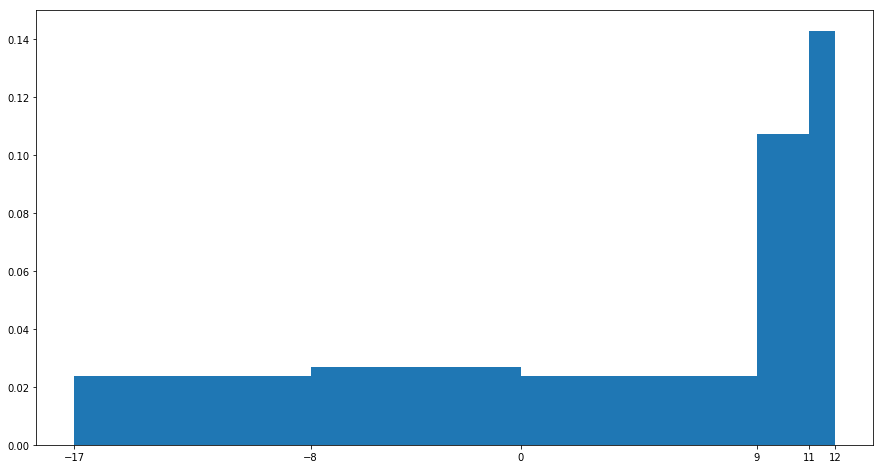
\includegraphics[width=\textwidth]{eqBinsZgled.png}
        \caption{Histogram množice $S$ z enakovrednimi stolpci. Zadnji stolpec vsebuje le 2 podatka, ostali pa 3.}
    \end{figure}

\end{zgled}